\begin{minipage}[t][\PosterLowerRowHeight][t]{\PosterHalfWidth}\vspace{0pt}
  \begin{PosterPanel}{\PosterLowerRowHeight}{8}{A LIMIT THAT REDISTRIBUTION CANNOT BEAT}
    \hyphenpenalty=10000\exhyphenpenalty=10000

    \noindent\begin{minipage}[t]{222mm}\vspace{0pt}
      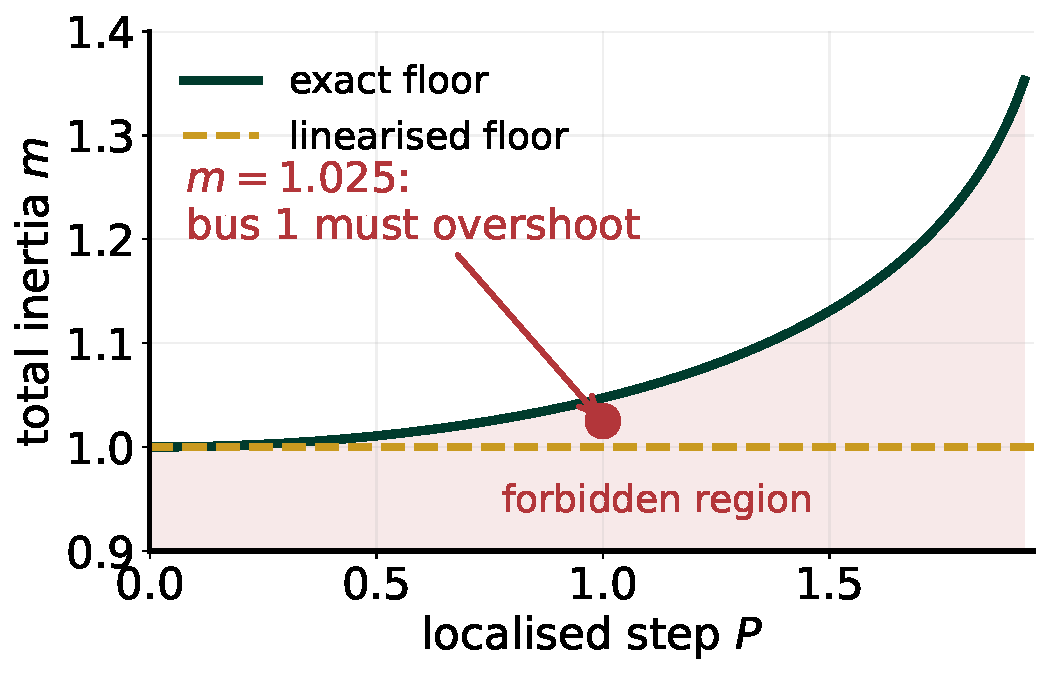
\includegraphics[width=220mm,height=104mm,keepaspectratio]{generated/figures/floor2.pdf}\par
      {\FigureSize Two-node nonlinear lossless network, localised step $P$. The exact floor is $\inf m=2\arcsin(P/2)/P$, equal to $\pi/3$ at $P=1$.\par}
    \end{minipage}\hfill%
    \begin{minipage}[t]{200mm}\vspace{0pt}
      {\FigureSize After a localised step, no local frequency can avoid crossing its final value unless total inertia exceeds a network floor:\par}
      {\EquationSize\color{IASBlue}\[
        m+\kappa>d_0^{2}\,(e_k-c)^{\top}\bar L_k^{\dagger}(e_k-c)
      \]}
      \vspace{-2mm}
      \begin{InWords}\InWordsLabel $\bar L_k$ is the secant-resistance graph between the event site $e_k$ and the primary response $c$. Moving inertia around, or adding damping that nets zero energy, cannot lower the floor.\end{InWords}
    \end{minipage}\par
    \vspace{3mm}
    {\FigureSize \textbf{Checked:} the area law matches a nonlinear simulation to six decimals (bus-1 area $-0.005549$ at $m=1.025$). \textbf{Scope:} the proof is for the reduced lossless class. On IEEE-39 the energy and area balance holds to $3\times10^{-10}$ MW, but the trajectory terms (ZIP load, losses, governor limits) are not yet bounded.\par}

  \end{PosterPanel}
\end{minipage}%
